\chapter{Implementation}
This chapter will describe the implementation of the entire system in the demonstrator.

\section{Platform}
To demonstrate the system, the RC car UTOR 8E from BSD racing was chosen. It is a 1/8 scale RC car with a steering servo, brushless DC motor, and most importantly, it was readily available from a local store.\\

For the demonstrator, it was decided to use the Zedboard on both vehicles for a number of reasons:
\begin{itemize}
\item The power supply connector for the EMC\textsuperscript{2}DP would have to be remade to be used in the vehicle.
\item Connections on the vehicles fitting the measurements of the Zedboard were already made.
\item Same BSP for both vehicles.
%\item The Zedboard was all around easier to work with
\end{itemize}

The car with all of its components can be seen in figure~\ref{fig:utor_overview}.

\begin{figure}[H]
\centering
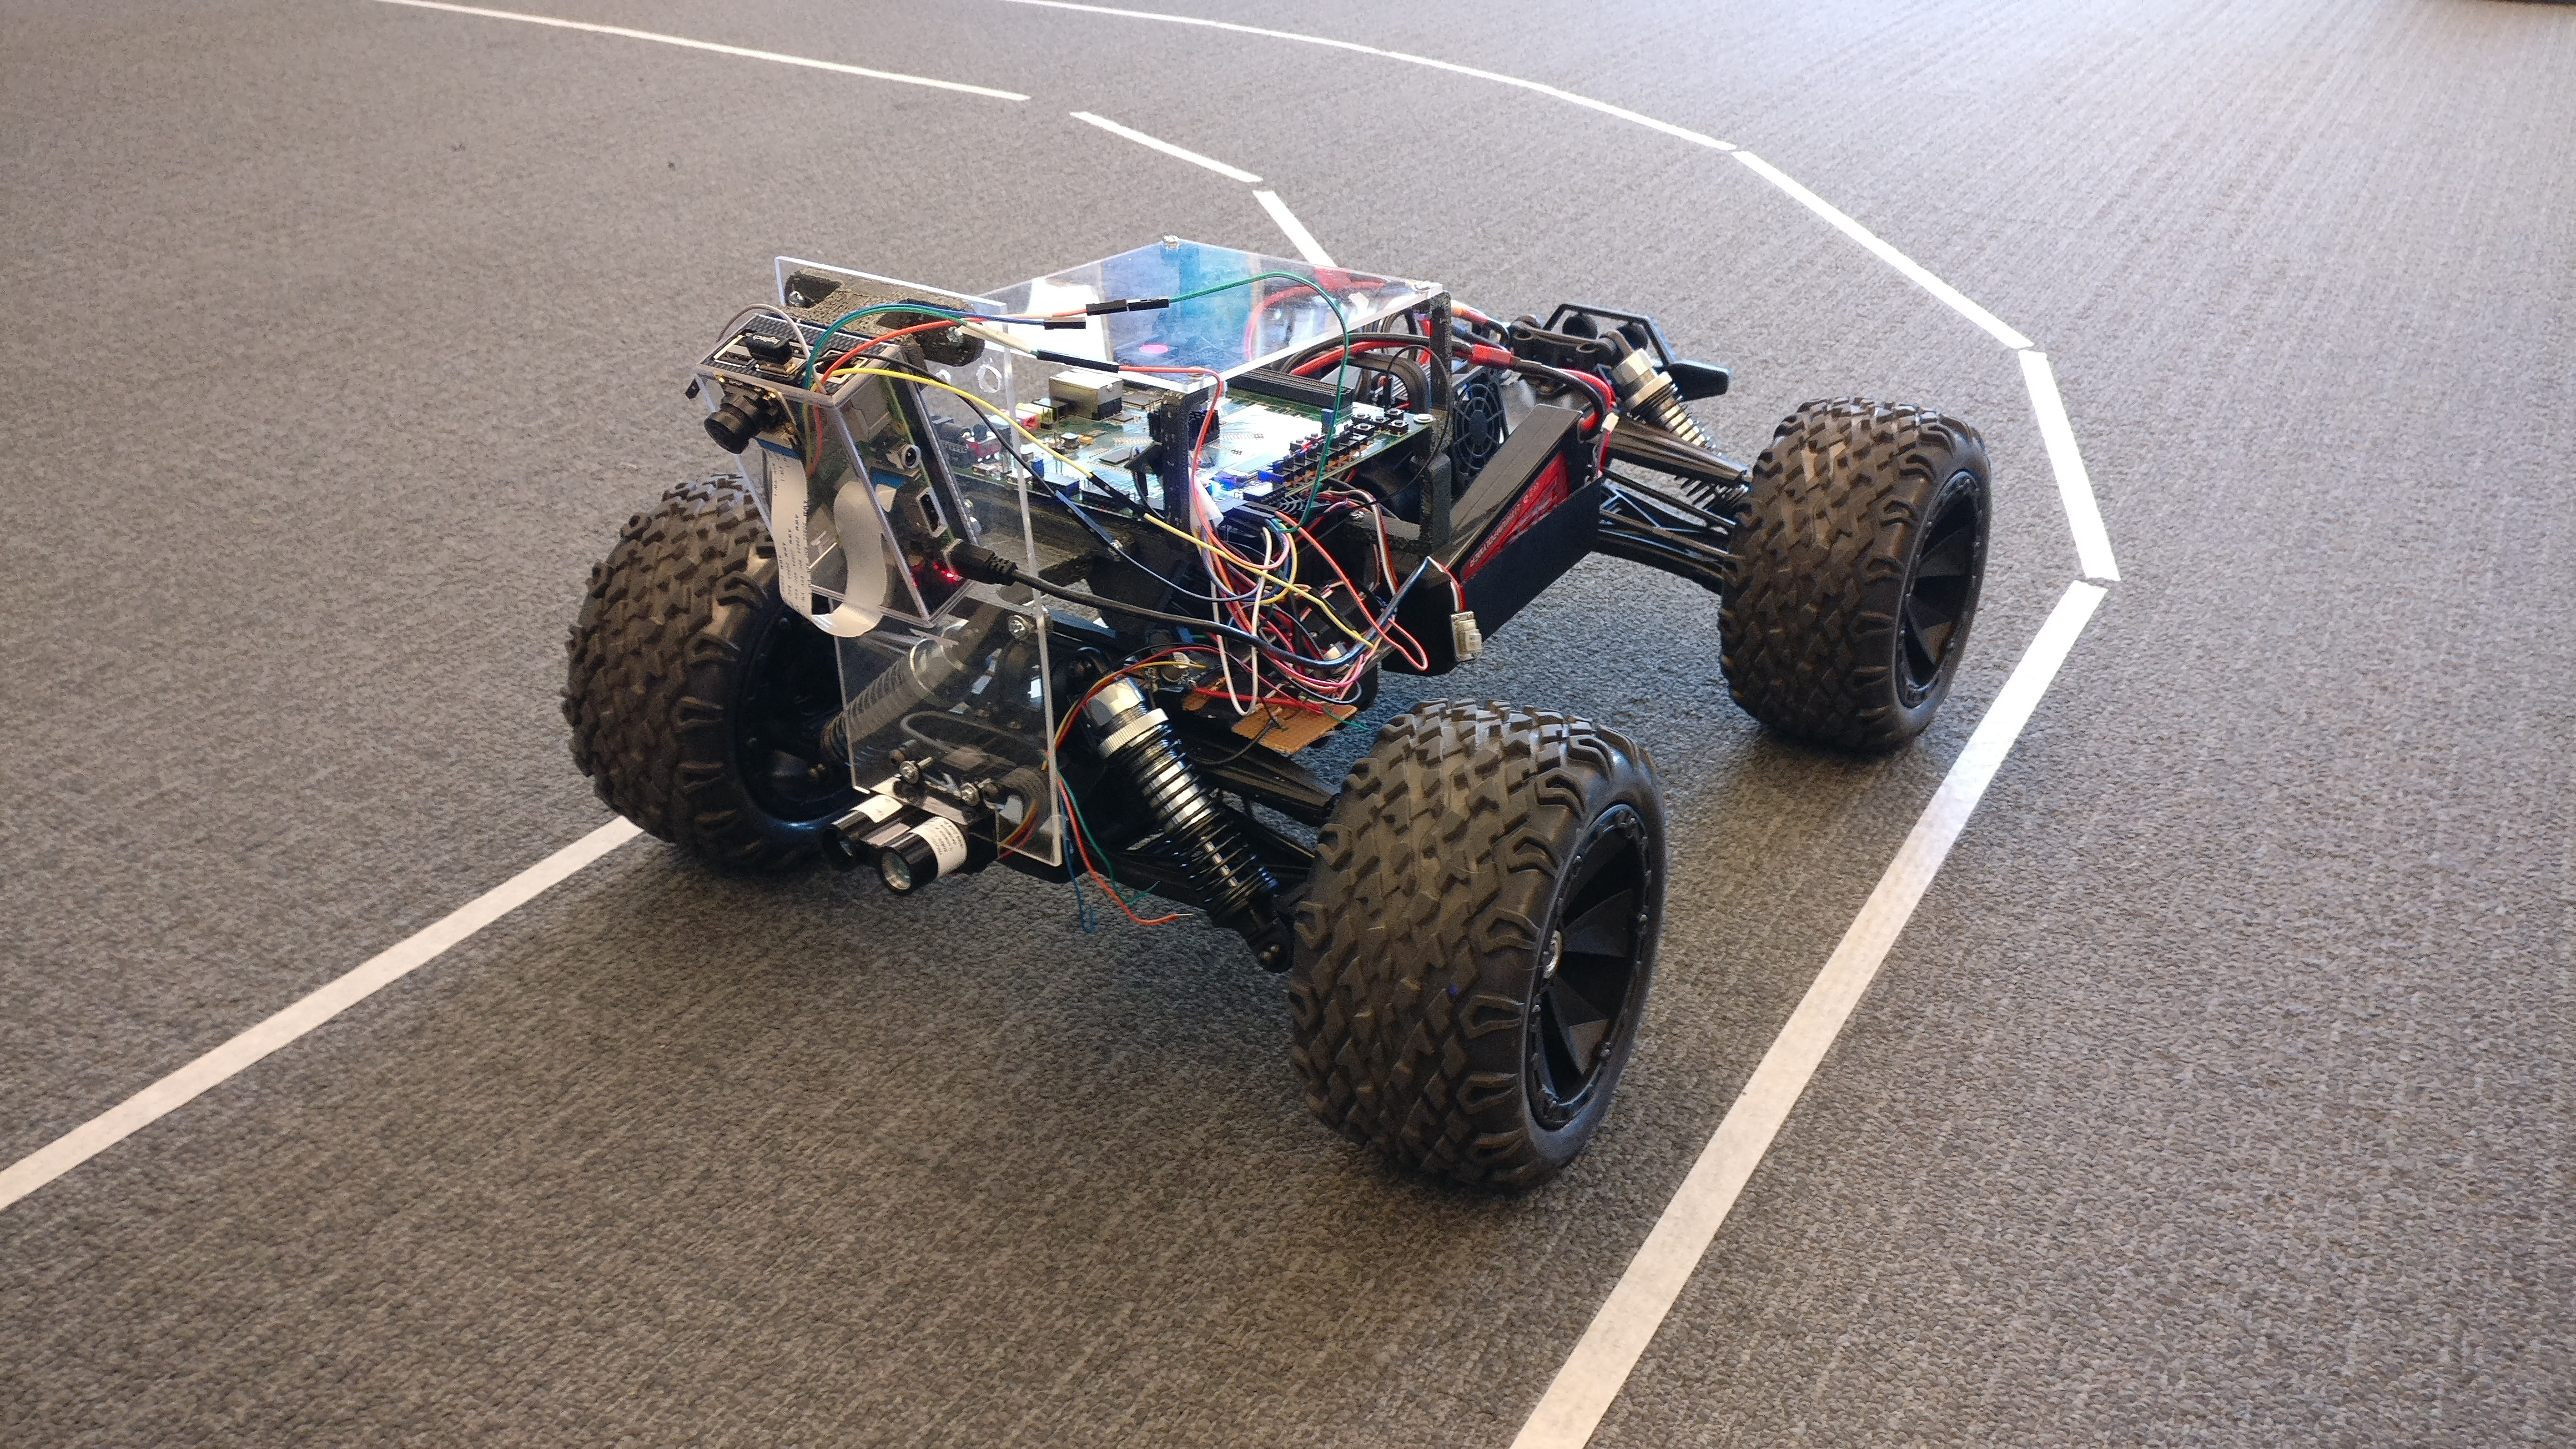
\includegraphics[width=\textwidth]{./img/implementation_utor.jpg}
\caption{One of the two vehicles on the test track. Visible in the picture is the LIDAR in the front, the Raspberry Pi and its camera. The Zedboard can be seen under the covering plastic glass.}
\label{fig:utor_overview}
\end{figure}

\subsection{Driver}
The driver for the motor and steering servo is controlled by a PWM signal with a frequency of 50~Hz. The speed is controlled by the pulse length of the PWM signal. This was tested with the hand-controller to see what PWM signals were received at the end points. Maximum and minimum high time measured was 2~ms and 1~ms, which at 50 Hz corresponds to a duty cycle of 10 and 5 \%. Depending on how high frequencies the driver could handle, the frequency could be increased without changing the high time, potentially up until a period of 0.02 seconds would make the maximum signal correspond to a duty cycle of 100\%.\\

This was tested, and gave somewhat expected results. The driver had some disturbances and gave maximum or minimum output sporadically when it shouldn't, with more disturbances at higher frequencies. It was decided that a frequency of 50 Hz would have to do.

\section{Electrical wiring}
The electrical power for all components on the car is sourced from the battery pack: two 7.4V batteries in parallel. Three voltage regulators are connected to the batteries to give power to other components. 

\begin{itemize}

\item 7.4V to 5V for LIDAR, Encoders and Raspberry Pi.

\item 7.4V to 5V for WiFi module.

\item 7.4V for DC input voltage for Zedboard. (Here the voltage regulator only acts as a filter.)

\end{itemize}

The WiFi module was put separately from the other 5V output since it draws too much current to be combined with the other components for one voltage regulator to handle. 

\section{RTOS tasks}
This section will describe the task implemented on the RTOS.

\subsection{Data aggregation}
The task \texttt{data\_aggregation()} is the task with the highest frequency in the system. It executes with a period of 1 ms, which the shortest period allowed in FMP. It reads the speed from each wheel as measured by the decoder, and determines if the road conditions are unsafe for platooning. It also filters speed and distance measurements through a low-pass filter to produce reliable data for the other tasks to use.

\subsection{Communication}
The task \texttt{communication()} reads V2V and I2V messages stored in a buffer on the FPGA. The messages are unpacked and forwarded to their intended destination task. Information from the other tasks are sent to the FPGA. The task \texttt{communication()} is bounded by the period of the larger communication loop and the period of \texttt{lateral\_control()} and \texttt{longitudinal\_control()}. It can only send messages with a period of 800 ms. Since the received messages are stored in a buffer on the FPGA, the task only needs to execute before every execution of \texttt{lateral\_control()} and \texttt{longitudinal\_control()}. This puts its period at 20~ms.

\subsection{Lateral control}
The task \texttt{lateral\_control()} receives angle and positional error of the vehicle in relation to the detected lane and computes a control signal via a PID controller. It also sends lane detection status to \texttt{longitudinal\_control()}. Due to the limitations by the PWM described earlier the control frequency was capped at 50 Hz, meaning a period of 20 ms.

\subsection{Longitudinal control}
Just like \texttt{lateral\_control()}, the period of \texttt{longitudinal\_control()} is 20 ms. The task consists of two PID controllers, one for CC and one for ACC (as described in chapter~\ref{sec:system_design}). The controller adds the control signal from the preceding vehicle to its own control signal if secure communication is established and the vehicles are in platoon/CACC mode. It also sends its control signal to the \texttt{communication()} task. If the lane detection status received from \texttt{lateral\_control()} indicates that no lane is detected, \texttt{longitudinal\_control()} stops the vehicle.

\section{GPOS}
Linux was run on the non-secure side. From the beginning there were ideas of hosting a video feed from the camera on the vehicle, but there was not nearly enough time to implement this. Instead, the Linux was running idle and was only used to navigate the file system to demonstrate that it was in fact up and running. 

\section{Processor scheduling}
The above tasks with their required frequencies resulted in the processor scheduling seen in figure~\ref{fig:rtsched}.

\begin{figure}[H]
\centering
\begin{RTGrid}[nonumbers=1]{6}{25}

%Data aggregation
\TaskNArrival{1}{0}{7}{4}
\TaskNExecDelta{1}{0}{1}{7}{4}

%Communication
\TaskArrival{2}{0}
\TaskRespTime{2}{0}{1}
\TaskExecution{2}{1}{2}

%Lateral control
\TaskArrival{3}{0}
\TaskRespTime{3}{0}{2}
\TaskExecution{3}{2}{3}

%Longitudinal control
\TaskArrival{4}{0}
\TaskRespTime{4}{0}{3}
\TaskExecution{4}{3}{4}

\TaskExecution{5}{4}{5}

%OS switch
\TaskNExecDelta{5}{6}{1}{7}{3}
\TaskNExecDelta{5}{8}{1}{7}{3}

%GPOS
\TaskRespTime{6}{0}{25}
\TaskExecution{6}{5}{6}
\TaskNExecDelta{6}{9}{4}{7}{2}
\TaskExecution{6}{23}{25}

\end{RTGrid}
\caption{Processor scheduling, not to scale.}\label{fig:rtsched}
\begin{tabular}{r@{: }l r@{: }l r@{: }l}
$\tau_1$ & Data aggregation & $\tau_2$ & Communication & $\tau_3$ & Lateral control\\
$\tau_4$ & Longitudinal control & $\tau_5$ & OS switch & $\tau_6$ & GPOS
\end{tabular}
\end{figure}

\section{Hardware functions}
This section will describe the implementation of the hardware functions, or FPGA IPs. For the entire Vivado block design showing the FPGA IPs and their interconnect, see Appendix.

\subsection{Pulse Width Modulation}
Two AXI Timer IPs were used to control the PWM signal to the motor and servo. Each AXI Timer has two internal timers, one timer setting the output high at the period specified, and one timer setting the output low after the start of the first timer, effectively creating a PWM signal. The resolution of the timers are 20 ns.

\subsection{LIDAR}
To read the distance to the preceding vehicle, Garmin LIDAR Lite v3 was used. Its technical specifications can be read in table~\ref{table:lidar}.

\begin{table}[H]
\centering
\begin{tabular}{|l|l|}
\hline
\textbf{Specification} & \textbf{Measurement}\\ \hline
Power & 5 Vdc nominal\\
 & 4.5 Vdc min., 5.5 Vdc max.\\ \hline
Current consumption & 105 mA idle\\
 & 135 mA continuous operation\\ \hline
User interface & I2C\\
 & PWM\\ \hline
Range & 40 m\\ \hline
Resolution & $\pm$1 cm\\ \hline
Accuracy $<$ 5 m & $\pm$2.5cm\\ \hline
Accuracy $\leq$ 5 m & $\pm$10 cm\\ \hline
Repetition rate & 50 Hz default\\
 & 500 Hz max\\ \hline
\end{tabular}
\caption{Specifications for Garmin LIDAR Lite v3.}
\label{table:lidar}
\end{table}

As can be seen in table~\ref{table:lidar}, there are two interface options for the LIDAR, I2C and PWM. The PWM interface was chosen. A hardware function was implemented on the FPGA to read the pulse width from the PWM signal. The length of the pulse width was counted and written on an AXI bus address, ready for the OS to be read and converted into a distance in cm. %The hardware code was written in VHDL and can be seen in Appendix~B.

\subsection{Encoders/Decoders}
To read the speed of each wheel, encoders with a resolution of 1024 ppr were used. To convert the signals from each encoder, hardware implemented decoders were written. The decoders read A and B pulses from each encoder and counted the time between each pulse to calculate the rotational speed of the wheels. This value was written on an AXI bus address for the OS to read. %The hardware code was written in VHDL and can be seen in Appendix~B.

\subsection{UART}
To communicate with the Raspberry Pi, the UART interface was used. The IP UART Lite with a baudrate of 115200 was implemented on the FPGA.

\subsection{MicroBlaze}
To handle the communication protocol, a processor in the form of a MicroBlaze was implemented on the FPGA. For more information, see the report by Lerander~\cite{lerander2017}.
